% !TEX program = pdflatex
% Overleaf-compatible. Self-contained: only stock packages.
% Figures live in ./figures/zebra_nav/ (see paper/README.md for how to regenerate).
\documentclass[11pt]{article}

\usepackage[margin=1in]{geometry}
\usepackage{graphicx}
\usepackage{booktabs}
\usepackage{makecell}
\usepackage{float}
\usepackage{amsmath}
\usepackage{amssymb}
\usepackage{xcolor}
\usepackage{caption}
\usepackage{subcaption}
\usepackage{enumitem}

\captionsetup{font=small, labelfont=bf}
\newcommand{\code}[1]{\texttt{#1}}

\title{\textbf{zebra\_nav}\\[2pt]
\large A POMDP navigation environment with a bridge / mine / detour
strategy choice, built as a substrate for mechanistic interpretability}
\author{}
\date{}

\begin{document}
\maketitle
\vspace{-2.2em}

\begin{abstract}\noindent
\textsc{zebra\_nav} is a small partially-observable navigation environment in
which an agent crosses open procedural terrain to reach a narrow goal door. The
direct route is blocked by obstacles the agent can deal with in three distinct
ways: \textbf{bridge} a lake (place wood on water), \textbf{mine} a mountain
(turn rock to grass), or \textbf{walk around} it. Impassable tree forests line
the top and bottom edges so the agent is funnelled through the obstacle-filled
middle, where it must repeatedly choose among the three strategies. The point of
the design is \emph{not} the navigation itself but the \textbf{internal computation
it induces}: under partial observation the agent must infer the shape and type of
the obstacle ahead (a \emph{belief}) and select a crossing strategy (an
\emph{action mode}). We train two agents on the identical task --- a recurrent PPO
baseline and a pure-JAX DreamerV3 world model --- both reaching $100\%$ success,
and use them as a testbed for probing and \textbf{steering} those belief and
strategy representations in activation space. The concrete target is to make an
agent that solves the task reliably but \textbf{never digs tunnels}, by
suppressing the ``mine'' strategy through an activation-space intervention rather
than an action mask.
\end{abstract}

\section{Idea and motivation}

We want a task that is (i) trivial to solve, so competence is not the bottleneck,
yet (ii) forces a small number of \emph{discrete, legible decisions} that depend
on a \emph{partially-observed latent} (the obstacle ahead). Such a task is an
ideal substrate for mechanistic interpretability: there should be a low-dimensional
\emph{belief} subspace (is the obstacle water or rock; how wide is it) and a
\emph{strategy} subspace (bridge vs.\ mine vs.\ detour) in the agent's recurrent
state, and we can test whether those subspaces are (a) linearly decodable and
(b) \emph{causally} steerable. The headline experiment is suppression: keep the
agent fully competent while removing one option (tunneling) by editing activations
--- the recurrent analogue of the ``cheese vector'' steering result on maze-solving
policy networks.

\section{Environment}

\paragraph{Tiles.} A $9$-tile symbolic vocabulary (no decorative classes, so the
decoder cannot interpolate phantom tiles):
\begin{center}\small
\begin{tabular}{@{}llll@{}}
\toprule
id & tile & role & behaviour\\
\midrule
0 & \code{GRASS}  & open ground & walkable (cost 1)\\
1 & \code{WATER}  & lake        & cross by \emph{bridging} (place $\to$ wood)\\
2 & \code{ROCK}   & mountain    & cross by \emph{mining} (mine $\to$ grass)\\
3 & \code{WOOD}   & placed bridge & walkable\\
4 & \code{TARGET} & goal door   & walkable; stepping on it wins\\
5 & \code{OOB}    & off-map pad & egocentric padding only\\
6 & \code{TREE}   & forest      & \textbf{impassable} (detour only)\\
7 & \code{SAND}   & water fringe & cosmetic, walkable like grass\\
8 & \code{DIRT}   & rock fringe  & cosmetic, walkable like grass\\
\bottomrule
\end{tabular}
\end{center}

\paragraph{Observation (POMDP).} An egocentric crop centred on the agent:
$\code{minimap}\in\{0,\dots,8\}^{V\times V}$ with $V=21$ (off-map cells padded with
\code{OOB}), plus a scalar vector $\code{scalars}\in\mathbb{R}^{5}=[\textsc{facing}
\text{ one-hot}(4),\ \text{step}/\text{max}]$. The agent never sees the whole map,
so the size/type of an obstacle must be \emph{inferred} as it approaches.

\paragraph{Actions.} \code{Discrete(6)}: up / down / left / right (a move also sets
\textsc{facing}), \code{PLACE} (bridge the water cell in front: $\code{WATER}\to
\code{WOOD}$), and \code{MINE} (mine the rock cell in front: $\code{ROCK}\to
\code{GRASS}$). Trees can never be removed.

\section{Task and procedural maps}

Maps are $32\times64$, generated by a domain-warped fractal heightmap thresholded
into lakes (\code{WATER}) and mountains (\code{ROCK}) with cosmetic \code{SAND}/
\code{DIRT} fringes; the left/right edge columns are kept obstacle-free. The
\textbf{spawn} is the centre of the left edge and the \textbf{goal} is a $3$-cell
central door on the right wall ($\code{goal\_half}=1$). Crucially, impassable
\textbf{tree forests are biased heavily toward the top and bottom rows} (about a
$7\!:\!1$ edge-to-middle ratio), which walls off the trivial ``hug the wall to the
door'' route and forces traversal through the obstacle-filled centre.
Figure~\ref{fig:maps} shows the curated validation set.

\begin{figure}[H]
\centering
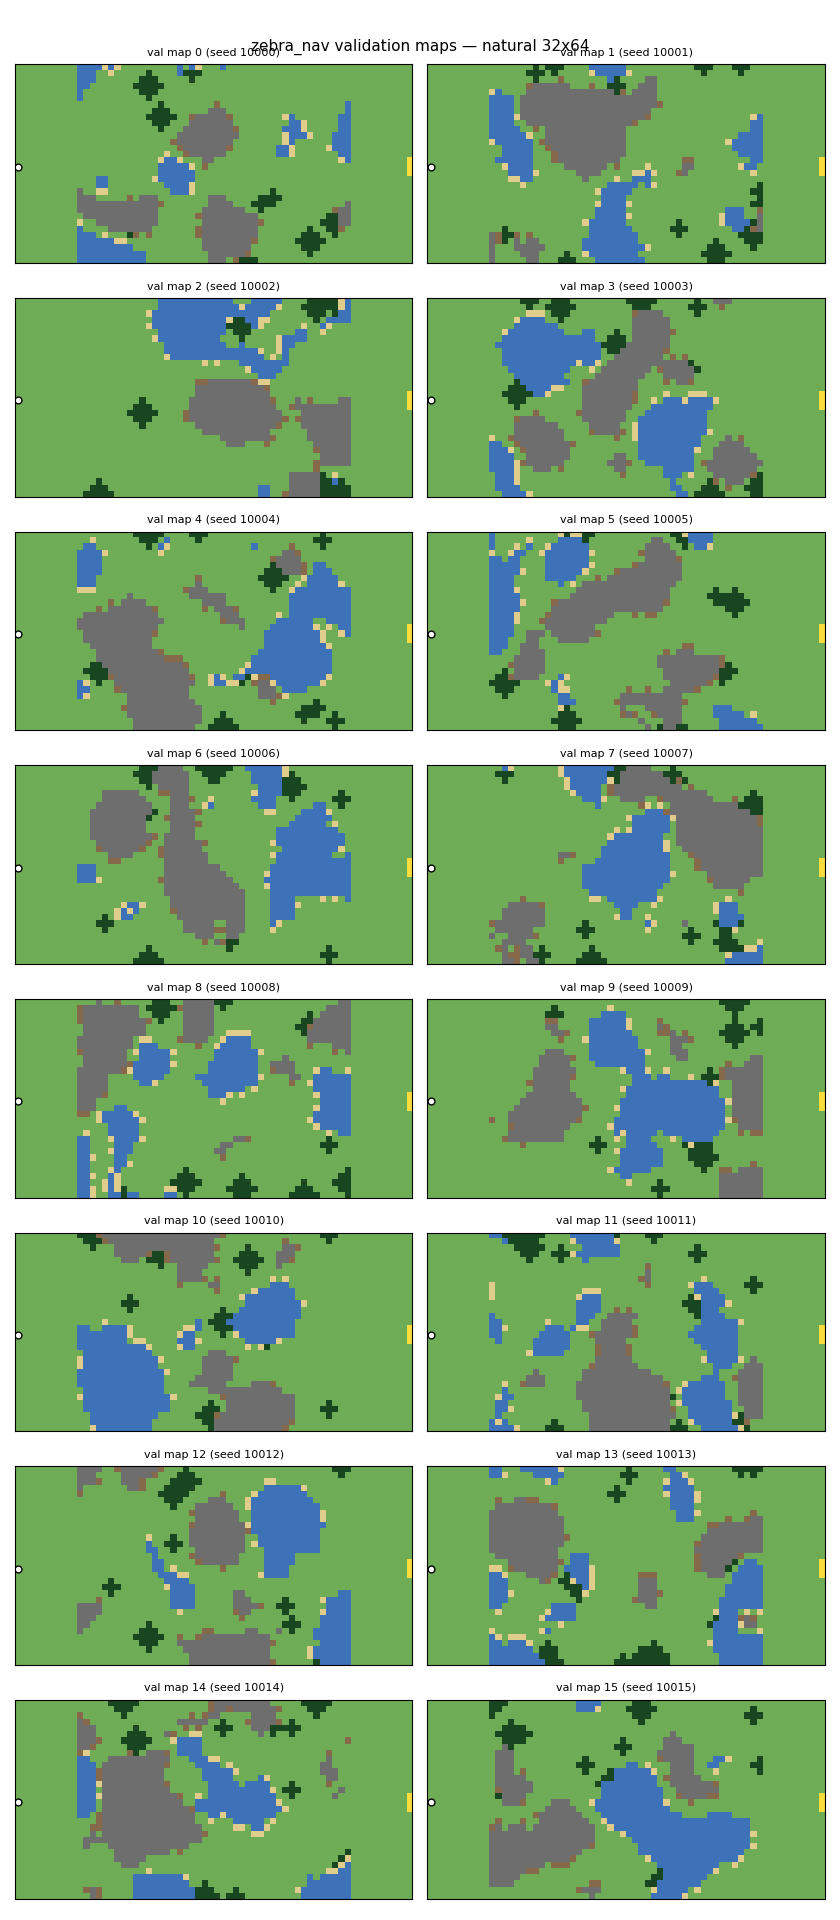
\includegraphics[width=0.86\linewidth]{figures/zebra_nav/maps.png}
\caption{The 16 validation maps. White dot = spawn (centre-left); yellow = the
3-cell goal door (centre-right). Blue lakes (bridge), grey mountains (mine), dark
forests clustered along the top/bottom edges (detour). The demo plays these exact
maps.}
\label{fig:maps}
\end{figure}

\paragraph{Why this geometry.} An earlier variant used the \emph{whole} right wall
as the goal; with a free top/bottom border the cheapest route is to hug an edge and
sprint right, and both agents collapsed to wall-hugging with no obstacle crossing.
Making the goal a narrow central door \emph{and} foresting the edges restores the
intended behaviour: the agent must go through the middle and repeatedly choose
bridge / mine / detour. The strategy mix is therefore a property of the map
geometry, not of the exploration schedule.

\section{Reward}

A move-minimising shaped reward with no per-strategy bias:
\[
r_t \;=\; \underbrace{-0.01}_{\text{slack}}
\;+\;\underbrace{\text{shaping}_t}_{\phi=-\,\text{ctg}}
\;+\;\underbrace{3.0\cdot\mathbb{1}[\text{reach door}]}_{\text{terminal}},
\qquad
\text{shaping}_t = 0.015\,\big(\text{ctg}_{t-1}-\gamma\,\text{ctg}_t\big),
\]
with $\gamma=0.997$. The potential $\phi=-\text{ctg}$ uses a \textbf{min-action
cost-to-go}: entering \code{WATER}/\code{ROCK} costs $2$ (build + move), walkable
tiles cost $1$, and \code{TREE} is impassable; \code{ctg} is computed once at reset
by Dijkstra seeded from the goal cell. With per-build cost $0$, crossing and
detouring are valued purely by total action count, so which strategy the agent
picks at a given obstacle is driven by geometry (is bridging/mining shorter than
going around?), exactly the decision we want to study.

\section{Agents}

Both agents train on the \emph{same} task to a shared metric schema. The PyTorch
PPO env (\code{ZebraNavEnv}) and the pure-JAX env (\code{ZebraNavJaxEnv}) are
proven bit-for-bit equivalent (a parity test asserts identical obs / reward /
termination over thousands of steps), so the DreamerV3 world model trains on
exactly the task the PPO agent does.

\begin{description}[leftmargin=1.2em]
\item[PPO + GRU.] A tile-embedding CNN with CoordConv $\to$ MLP $\to$ GRU
($128$ hidden) $\to$ \{categorical actor, value\}. The $128$-d GRU state is the
POMDP belief carrier and the primary probing target. Entropy $0.045$, no
annealing (keeps the stochastic policy spread out).
\item[DreamerV3 (25M).] The in-tree pure-JAX \code{purejaxwm} library: a 4-block
MLP encoder/decoder on the flat $V^2+5$ vector obs (the minimap is symbolic, so no
CNN), a block-GRU RSSM with discrete latents, TwoHot reward/value heads, RetNorm
actor scaling. Paper-aligned defaults ($\gamma{=}0.997$, $\lambda{=}0.95$,
$\text{lr}{=}4\mathrm{e}{-5}$).
\end{description}

\begin{center}\small
\begin{tabular}{@{}lccc@{}}
\toprule
agent & success & episode return & episode length\\
\midrule
PPO + GRU      & $100\%$ & ${\approx}3.3$ & ${\approx}92$\\
DreamerV3 (25M) & $100\%$ & ${\approx}3.4$ & ${\approx}95$\\
\bottomrule
\end{tabular}
\end{center}

\section{Behaviour: stochastic rollouts}

Figure~\ref{fig:grids} overlays $200$ stochastic rollouts per map for each agent.
The forests pin the paths into a central corridor; within it the agents bridge
(red), mine (yellow), and detour around the larger masses. Figure~\ref{fig:strat}
isolates one clean rollout of each strategy from the PPO agent --- the three
behaviours we want to find and manipulate internally.

\begin{figure}[H]
\centering
\begin{subfigure}{0.49\linewidth}\centering

\includegraphics[width=\linewidth]{figures/zebra_nav/ppo_traj.png}
\caption{PPO + GRU}
\end{subfigure}\hfill
\begin{subfigure}{0.49\linewidth}\centering
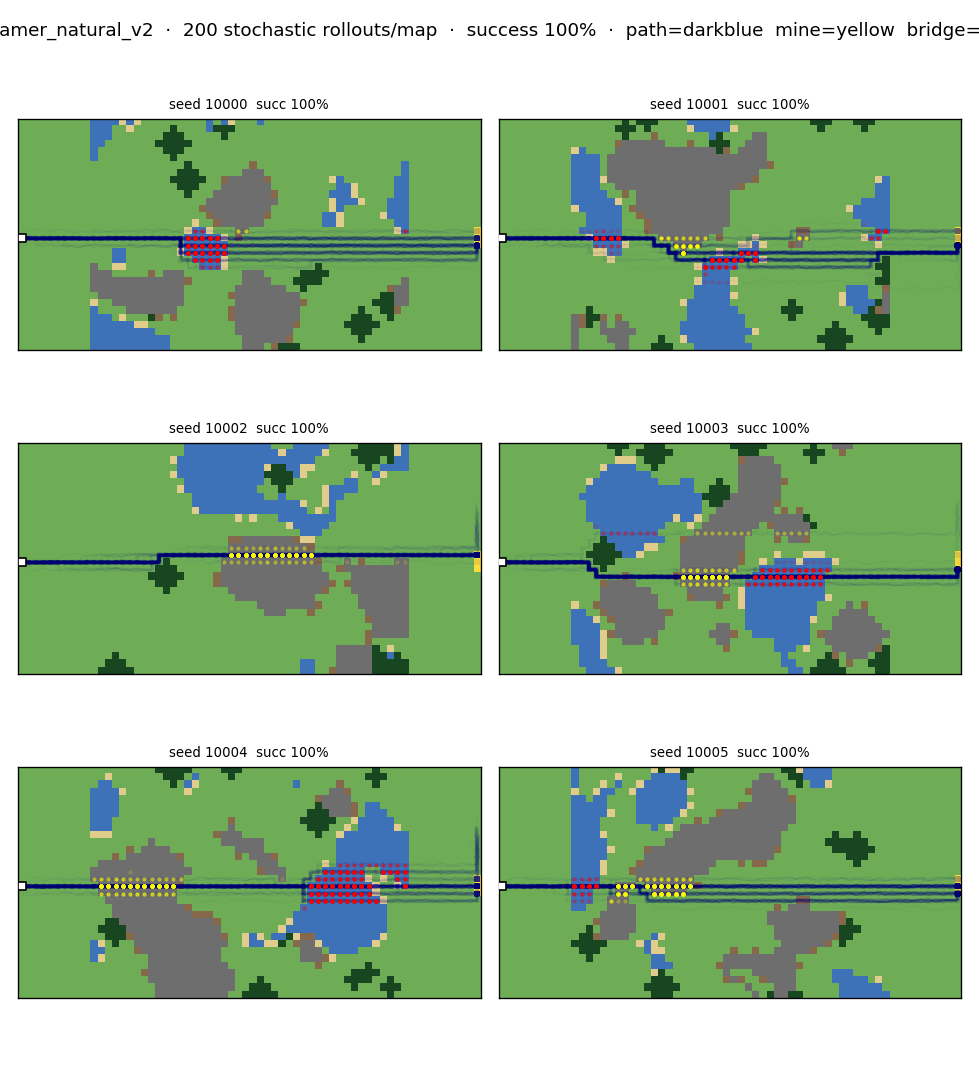
\includegraphics[width=\linewidth]{figures/zebra_nav/dreamer_traj.png}
\caption{DreamerV3}
\end{subfigure}
\caption{$200$ stochastic rollouts per map. path = dark blue, \textcolor{red}{bridge
= red}, \textcolor{orange}{mine = yellow}. Both agents funnel through the
forest-walled central corridor and cross obstacles there.}
\label{fig:grids}
\end{figure}

\begin{figure}[H]
\centering

\includegraphics[width=0.95\linewidth]{figures/zebra_nav/strategy_examples.png}
\caption{One stochastic rollout per strategy (PPO agent). \textbf{Avoid}: detours
around a rock+lake (no build). \textbf{Bridge}: places wood to cross a lake.
\textbf{Tunnel}: mines through rock. Across sampled rollouts the mix is roughly
avoid:bridge:tunnel $\approx$ 1:1.6:0.9, so all three modes are well represented.}
\label{fig:strat}
\end{figure}

\section{DreamerV3 imagination}

Because DreamerV3 learns a world model, we can roll it forward \emph{in
imagination} (latent rollouts under the actor, no environment) and decode each
imagined latent back to an egocentric view. Figure~\ref{fig:dream} plays such a
dream, decoded to Crafter sprites: warmup frames are real, then the model imagines
moving and crossing obstacles, predicting coherent grass/water/rock/tree terrain.

\begin{figure}[H]
\centering
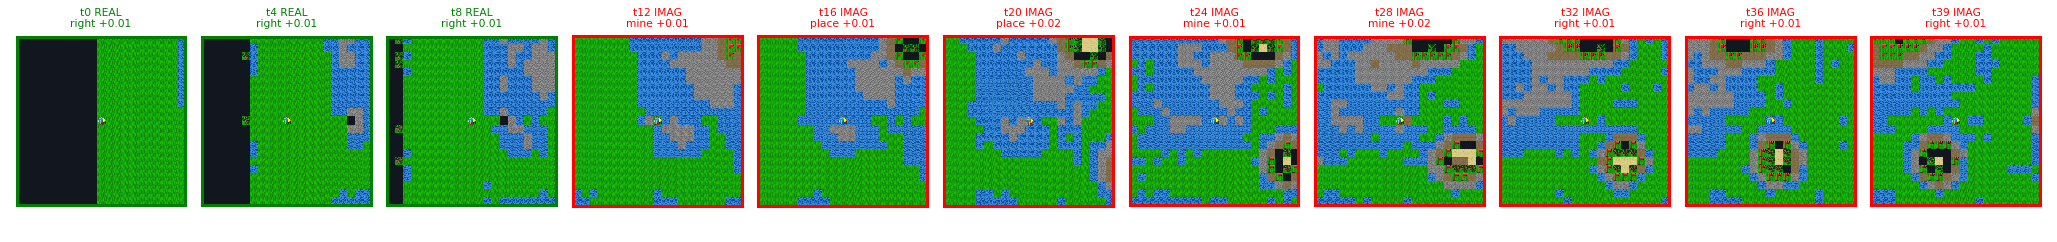
\includegraphics[width=\linewidth]{figures/zebra_nav/dreamer_imagine_strip.png}
\caption{A DreamerV3 imagined rollout decoded to sprites (green border = real
warmup, red = open-loop imagination). The world model imagines coherent terrain
--- including the edge tree bands --- and dreams mining/placing through the
middle.}
\label{fig:dream}
\end{figure}

\paragraph{An encoding caveat (relevant to probing).} The Dreamer obs encodes the
minimap as a single ordinal scalar per cell ($\text{tile\_id}/\text{NUM\_TILES}$)
and the decoder \emph{regresses} it. Reconstructions are therefore blurry and
\emph{not} a categorical tile-belief; a cleaner design (one-hot channels +
per-cell softmax decoder with cross-entropy) would make tile beliefs a crisp probe
target. The PPO agent already uses a proper tile \emph{embedding}.

\section{Mechanistic-interpretability plan}

The agents above are the substrate. The intended programme:
\begin{enumerate}[leftmargin=1.4em]
\item \textbf{Activation dataset.} Fix one or two maps, sample many stochastic
trajectories (logging seed + full metadata), and record the GRU state $h_t$ (and
the pre-recurrent encoder embedding) at every step, labelled with the
ground-truth belief (obstacle type/size ahead) and the committed strategy
(avoid / bridge / tunnel) at each obstacle.
\item \textbf{Probe.} Fit linear probes / difference-of-means directions for the
belief and strategy variables; report decoding accuracy by site, and validate with
unsupervised structure (PCA / clustering).
\item \textbf{Steer.} Add / clamp those directions during fresh rollouts and
measure the causal behavioural change (a probe that decodes but does not steer is
suspect).
\item \textbf{Suppress.} Derive the ``mine'' direction from the \emph{decision}
contrast (mined vs.\ went-around on the same rock obstacle), apply it conditionally,
and verify the agent re-routes via its own bridge/detour policy rather than
failing --- i.e.\ a competent agent that \textbf{never digs tunnels}, achieved in
activation space.
\end{enumerate}

\paragraph{Reproduce.} Train: \code{scripts/train\_ppo\_zebra.py --config
models/zebra\_nav/natural\_centergoal3.yaml} and \code{scripts/dreamerv3\_zebra\_nav.py
--size 25M}. Visualise: \code{scripts/zebra\_traj\_grid.py},
\code{scripts/zebra\_strategy\_examples.py}, \code{scripts/viz\_dreamer\_zebra\_imagine.py}.
See \code{docs/zebra\_nav.md} and \code{docs/codebase\_map.md}.

\end{document}
